

\paragraph*{Processes}
Let
\begin{inline}
   \item $\mprc,\mprc', \mqrc$ range over processes
   %
   \item \pvar\ range over process variables
   %
   \item \setA\ be an ordered set of message labels
   %
   \item \setC\ be an ordered set of session channels
   %
   \item \psetX\ be the set of local clocks (distinct to the set of clocks \setX\ used in the syntax of types)
   %
\end{inline}

In definition that follows
\begin{inline}
   \item \epointp\ and \epointq\ are two endpoints
   %
   \item \pchan\ is a channel between two endpoints
   %
   \item \bool\ is a boolean condition
   %
   \item \pbuffer\ points to the head of a channels buffer (ordered chronologically)
   %
\end{inline}
\begin{equation*}
   % \hspace{-5ex}%
   \mproccescalc%
\end{equation*}
The following sections discusses all of the changes from the previous work of~\cite{Bocchi2019}. \REDO[i am unsure if i have formulated \opt\ correctly, will need to discuss]
\TODO[still need single actions even though they can be represented here?]
\TODO[is it wrong to enforce active() on actions?]

\subsection{New\TODO}

\subsubsection*{Choices and Options}
A process $\mprc=\mpchan\;\mopt$ describes that the channel \pchan\ will be used by one of the options taken in \opt.

\opt\ is structured

\begin{example}[Constructing Processes]
   Below is a modification of the type shown in~\cref{fig:motiv_example_producer_consumer_diagram}:
   \begin{equation*}
      \resizebox{\textwidth}{!}{$
            \mrec\,{{\mreclabel}^{Z}}%
            \,.\,%
            \left\{\def\arraystretch{1.7}%
            \begin{array}{l}%
               \mrecv\mathtt{ready}\,\left(1\leq x\leq 2,\,x\right)%
               \,.\,%
               \left\{\def\arraystretch{1.7}%
               \begin{array}{l}%
                  \msend\mathtt{latency}\,\left(y-x=2,\right)%
                  \,.\,%
                  {{\mreclabel}^{Z}}%
                  \,, \\%
                  %
                  %
                  \msend\mathtt{start}\,\left(x=2,\right)%
                  \,.\,%
                  \mrec\,{{\mreclabel}^{A}}%
                  \,.\,%
                  \left\{\def\arraystretch{1.7}%
                  \begin{array}{l}%
                     \msend\mathtt{cancel}\,\left(x\leq 2\right)%
                     \,.\,%
                     \mend%
                     \,, \\%
                     %
                     %
                     \mrecv\mathtt{done}\,\left(2\leq x\leq 5\right)%
                     \,.\,%
                     \msend\mathtt{ok}%
                     \,.\,%
                     \mend%
                     \,, \\%
                     %
                     %
                     \mrecv\mathtt{data}\,\left(2\leq x\leq 5\right)%
                     \,.\,%
                     {{\mreclabel}^{A}}%
                     \,, \\%
                     %
                     %
                     \mrecv\mathtt{error}\,\left(2\leq x\leq 6\right)%
                     \,.\,%
                     \msend\mathtt{restart}%
                     \,.\,%
                     {{\mreclabel}^{Z}}%
                     \,, \\%
                     %
                     %
                     \msend\mathtt{timeout}\,\left(6<x\right)%
                     \,.\,%
                     {{\mreclabel}^{Z}}%
                     %
                     %
                  \end{array}%
                  \right\}%
                  %
                  %
               \end{array}%
               \right\}%
               \,, \\%
               %
               %
               \msend\mathtt{close}\,\left(x=2.5\right)%
               \,.\,%
               \mend%
               %
               %
            \end{array}%
            \right\}%
         $}
   \end{equation*}

   Against a global clock $g$ (which can only be reset when a recursive call is made), the following graph can be constructed to represent the possible traces of viable sequences and timings of interactions:\newline
   \resizebox{\textwidth}{!}{%
      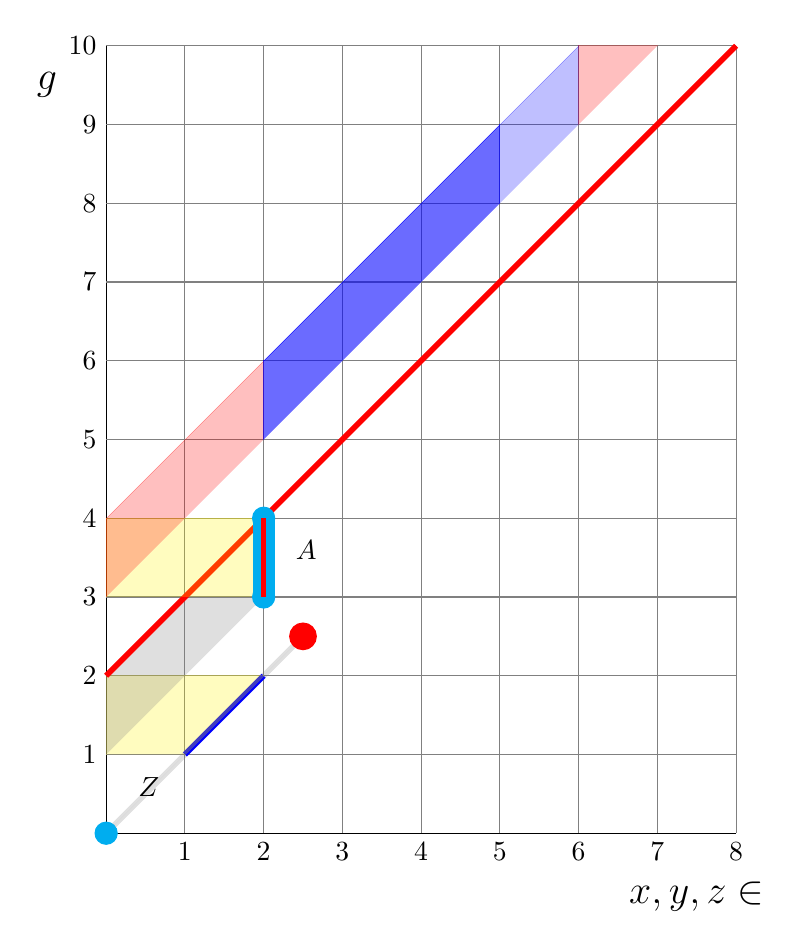
\begin{tikzpicture}
         % grid
         \draw (0,0) -- (8,0);%
         \draw (0,0) -- (0,10);%
         % draw horizontal
         \foreach \y in {1,...,10}%
            {%
               \draw[gray] (0,\y) -- (8,\y);%
               \node[left] at (0,\y) {\y};
            }%
         % draw vertical
         \foreach \x in {1,...,8}%
            {%
               \draw[gray] (\x,0) -- (\x,10);%
               \node[below] at (\x,0) {\x};
            }%

         % complete trace
         \filldraw [gray, opacity = 0.25, line width = 2pt]%
         (0,0) -- (2.5,2.5);%
         \filldraw [blue, opacity = 1, line width = 2pt]% ready
         (2,2) -- (1,1);%
         \filldraw [yellow, opacity = 0.25, line width = 0pt]% reset
         (0,1) -- (0,2) -- (2,2) -- (1,1);%
         \filldraw [gray, opacity = 0.25, line width = 0pt]%
         (0,1) -- (0,2) -- (1,3) -- (2,3);%
         \filldraw [red, opacity = 1, line width = 2pt]% latency
         (0,2) -- (8,10);%

         \filldraw [yellow, opacity = 0.25, line width = 0pt]% reset
         (0,3) -- (0,4) -- (2,4) -- (2,3);%
         \filldraw [red, opacity = 0.25, line width = 0pt]% cancel
         (0,3) -- (0,4) -- (2,6) -- (2,5);%
         \filldraw [blue, opacity = 0.25, line width = 0pt]% done
         (2,5) -- (2,6) -- (5,9) -- (5,8);%
         \filldraw [blue, opacity = 0.25, line width = 0pt]% data
         (2,5) -- (2,6) -- (5,9) -- (5,8);%
         \filldraw [blue, opacity = 0.25, line width = 0pt]% error
         (2,5) -- (2,6) -- (6,10) -- (6,9);%
         \filldraw [red, opacity = 0.25, line width = 0pt]% timeout
         (6,9) -- (6,10) -- (7,10);%

         % def z
         \draw[fill, cyan] (0,0) circle (4pt);
         \node[right] at (0.2, 0.5) {\Large $\mrec\,{{\mreclabel}^{Z}}$};

         % def a
         \draw[fill, cyan] (2,3) circle (4pt);
         \draw[fill, cyan] (2,4) circle (4pt);
         \filldraw [cyan, line width = 8pt] (2,3) -- (2,4);
         \node[right] at (2.2,3.5) {\Large $\mrec\,{{\mreclabel}^{A}}$};

         % send start
         \filldraw [red, opacity = 1, line width = 2pt]% start
         (2,4) -- (2,3);%

         % send close
         \filldraw [red, opacity = 1, line width = 2pt]%
         (2.5,2.5) circle (4pt);

         % axis labels
         \node[below] at (7.5,-0.5) {\Large $x,y,z\in\msetX$};
         \node[left] at (-0.5, 9.5) {\Large $g$};

         % % table of clock values: g
         % \node at (9, 10.5) {\Large $g$};
         % \node at (9, 10) {$10$};
         % \node at (9, 9) {$9$};
         % \node at (9, 8) {$8$};
         % \node at (9, 7) {$7$};
         % \node at (9, 6) {$6$};
         % \node at (9, 5) {$5$};
         % \node at (9, 4) {$4$};
         % \node at (9, 3) {$3$};
         % \node at (9, 2) {$2$};
         % \node at (9, 1) {$1$};
         % \node at (9, 0) {$0$};
         % % table of clock values: x
         % \node at (10, 10.5) {\Large $x$};
         % \node at (10, 10) {$(6,7)$};
         % \node at (10, 9) {$(5,6)$};
         % \node at (10, 8) {$(4,5)$};
         % \node at (10, 7) {$(3,4)$};
         % \node at (10, 6) {$(2,3)$};
         % \node at (10, 5) {$(1,2)$};
         % \node at (10, 4) {$2\mapsto 0$};
         % \node at (10, 3) {$\begin{array}{c}(1,2)\\2\mapsto 0\end{array}$};
         % \node at (10, 2) {$\begin{array}{c}(1,2)\\2\mapsto 0\end{array}$};
         % \node at (10, 1) {$1\mapsto 0$};
         % \node at (10, 0) {$0$};
         % % table of clock values: y
         % \node at (11, 10.5) {\Large $y$};
         % \node at (11, 10) {$10$};
         % \node at (11, 9) {$9$};
         % \node at (11, 8) {$8$};
         % \node at (11, 7) {$7$};
         % \node at (11, 6) {$6$};
         % \node at (11, 5) {$5$};
         % \node at (11, 4) {$4$};
         % \node at (11, 3) {$3$};
         % \node at (11, 2) {$2$};
         % \node at (11, 1) {$1$};
         % \node at (11, 0) {$0$};
      \end{tikzpicture}
   }

   Using the above graph, the following decision diagram can be extracted\TODO[work in progress]:\newline
   % \resizebox{\textwidth}{!}{%
   \resizebox{!}{20cm}{%
      \begin{tikzpicture}[
            every node/.style={xshift=0mm,yshift=0mm,draw,rectangle,rounded corners,fill=gray!20},
            %
            edge from parent/.style={
                  draw,->,
                  nodes={fill=blue!20,rectangle}
               },
            %
            end/.style={
                  nodes={xshift=0mm,yshift=0mm,fill=black,text=white,circle},
                  level distance=20mm
               },
            %
            Zdef/.style={
                  nodes={xshift=0mm,yshift=0mm,fill=green!40,ellipse},
                  edge from parent/.style={
                        midway,draw,->,
                        nodes={fill=green!30,rectangle,xshift=0mm,yshift=0mm}
                     },
                  level distance=30mm
               },
            %
            Zrec/.style={
                  nodes={xshift=0mm,yshift=0mm,fill=green!60,ellipse},
                  edge from parent/.style={
                        midway,draw,->,
                        nodes={fill=green!50,rectangle,xshift=0mm,yshift=0mm}
                     },
                  level distance=35mm
               },
            %
            Adef/.style={
                  nodes={xshift=0mm,yshift=0mm,fill=orange!40,ellipse},
                  edge from parent/.style={
                        midway,draw,->,
                        nodes={fill=orange!30,rectangle,xshift=0mm,yshift=0mm}
                     },
                  level distance=30mm
               },
            %
            Arec/.style={
                  nodes={xshift=0mm,yshift=0mm,fill=orange!60,ellipse},
                  edge from parent/.style={
                        midway,draw,->,
                        nodes={fill=orange!50,rectangle,xshift=0mm,yshift=0mm}
                     },
                  level distance=35mm
               },
            % general actions
            act/.style={
                  nodes={xshift=0mm,yshift=0mm,fill=white,rectangle,rounded corners},
                  edge from parent/.style={
                        draw,->,
                        nodes={fill=cyan!20,rectangle,xshift=0mm,yshift=2mm}
                     },
                  level distance=40mm
               },
            % middle actions in options
            optact/.style={
                  nodes={xshift=0mm,yshift=0mm,fill=white,rectangle,rounded corners},
                  edge from parent/.style={
                        draw,->,
                        nodes={fill=cyan!20,rectangle,xshift=0mm,yshift=0mm}
                     },
                  level distance=45mm
               },
            % always actions
            allact/.style={
                  nodes={xshift=0mm,yshift=0mm,fill=white,rectangle,rounded corners},
                  edge from parent/.style={
                        draw,->,
                        nodes={fill=cyan!20,rectangle,xshift=0mm,yshift=0mm}
                     },
                  level distance=35mm
               },
            % options
            opt/.style={
                  nodes={xshift=0mm,yshift=0mm,fill=magenta!40,diamond},
                  edge from parent/.style={
                        midway,draw,->,
                        nodes={fill=magenta!20,rectangle,xshift=0mm,yshift=0mm}
                     },
                  level distance=48mm
               },
            % nested options
            subopt/.style={
                  nodes={xshift=0mm,yshift=0mm,fill=magenta!40,diamond},
                  edge from parent/.style={
                        midway,draw,->,
                        nodes={fill=magenta!20,rectangle,xshift=0mm,yshift=0mm}
                     },
                  level distance=40mm
               }
         ]
         % root
         \node[act] {$
               \begin{array}{c}
                  g=0 \\% g
                  x=0 \\% x
                  y=0 % y
               \end{array}
            $}
         % def z
         child[Zdef] {
               node {$
                        \begin{array}{c}
                           g=0 \\% g
                           x=0 \\% x
                           y=0 % y
                        \end{array}
                     $}
               % recv ready
               child[act,grow=south west] {
                     node {$
                              \begin{array}{c}
                                 1\leq g\leq 2 \\% g
                                 x=0           \\% x
                                 1\leq y\leq 2 % y
                              \end{array}
                           $}
                     % send latency
                     child[act,grow=south west] {
                           node {$
                                    \begin{array}{c}
                                       2\leq g< 3 \\% g
                                       0\leq x< 2 \\% x
                                       2\leq y< 3 % y
                                    \end{array}
                                 $}
                           % rec z
                           child[Zrec] {
                                 node {$
                                          \begin{array}{c}
                                             g=0 \\% g
                                             x=0 \\% x
                                             y=0 % y
                                          \end{array}
                                       $}
                                 %
                                 edge from parent
                                 node {$
                                          {{\mreclabel}^{Z}}
                                       $}
                              }
                           %
                           edge from parent
                           node[left] {$
                                    \begin{array}{c}
                                       \msend\mathtt{latency}
                                       \\
                                       y-x=2
                                    \end{array}
                                 $}
                        }
                     % send latency or start
                     child[opt,grow=south] {
                           node {$
                                    \begin{array}{c}
                                       3\leq g\leq 4 \\% g
                                       x=2           \\% x
                                       3\leq y\leq 4 % y
                                    \end{array}
                                 $}
                           % send latency
                           child[act,grow=south west]  {
                                 node {$
                                          \begin{array}{c}
                                             3\leq g\leq 4 \\% g
                                             x=2           \\% x
                                             3\leq y\leq 4 % y
                                          \end{array}
                                       $}
                                 % rec z
                                 child[Zrec] {
                                       node {$
                                                \begin{array}{c}
                                                   g=0 \\% g
                                                   x=0 \\% x
                                                   y=0 % y
                                                \end{array}
                                             $}
                                       %
                                       edge from parent
                                       node {$
                                                {{\mreclabel}^{Z}}
                                             $}
                                    }
                                 % label
                                 edge from parent
                                 node[left] {$
                                          \begin{array}{c}
                                             \msend\mathtt{latency}
                                             \\
                                             y-x=2
                                          \end{array}
                                       $}
                              }
                           % send start
                           child[act,grow=south east]  {
                                 node {$
                                          \begin{array}{c}
                                             3\leq g\leq 4 \\% g
                                             x=0           \\% x
                                             3\leq y\leq 4 % y
                                          \end{array}
                                       $}
                                 % def a
                                 child[Adef,grow=south] {
                                       node {$
                                                \begin{array}{c}
                                                   3\leq g\leq 4 \\% g
                                                   x=0           \\% x
                                                   3\leq y\leq 4 % y
                                                \end{array}
                                             $}
                                       % send cancel
                                       child[act,grow=south west] {
                                             node {$
                                                      \begin{array}{c}
                                                         3\leq g\leq 6 \\% g
                                                         0\leq x\leq 2 \\% x
                                                         3\leq y\leq 6 % y
                                                      \end{array}
                                                   $}
                                             % end
                                             child[end] {
                                                   node {$\mend$}
                                                }
                                             %
                                             edge from parent
                                             node[left] {$
                                                      \begin{array}{c}
                                                         \msend\mathtt{cancel}
                                                         \\
                                                         x\leq 2
                                                      \end{array}
                                                   $}
                                          }
                                       % recv done, data or error
                                       child[opt,grow=south] {
                                             node {$
                                                      \begin{array}{c}
                                                         5< g\leq 9 \\% g
                                                         2< x\leq 5 \\% x
                                                         5< g\leq 9 % y
                                                      \end{array}
                                                   $}
                                             % recv done, data or error
                                             child[subopt,grow=south west] {
                                                   node {$
                                                            \begin{array}{c}
                                                               5< g\leq 9 \\% g
                                                               2< x\leq 5 \\% x
                                                               5< g\leq 9 % y
                                                            \end{array}
                                                         $}
                                                   % recv done
                                                   child[optact,grow=south west] {
                                                         node {$
                                                                  \begin{array}{c}
                                                                     5< g\leq 9 \\% g
                                                                     2< x\leq 5 \\% x
                                                                     5< g\leq 9 % y
                                                                  \end{array}
                                                               $}
                                                         % send ok
                                                         child[allact] {
                                                               node {$
                                                                        \begin{array}{c}
                                                                           5< g\leq 9 \\% g
                                                                           2< x\leq 5 \\% x
                                                                           5< g\leq 9 % y
                                                                        \end{array}
                                                                     $}
                                                               % end
                                                               child[end] {
                                                                     node {$\mend$}
                                                                  }
                                                               %
                                                               edge from parent
                                                               node[right] {$\msend\mathtt{ok}$}
                                                            }
                                                         %
                                                         edge from parent
                                                         node[left] {$
                                                                  \begin{array}{c}
                                                                     \mrecv\mathtt{done},
                                                                     \\
                                                                     2<x\leq 5
                                                                  \end{array}$}
                                                      }
                                                   % recv data
                                                   child[optact,grow=south,level distance=45mm] {
                                                         node {$
                                                                  \begin{array}{c}
                                                                     5< g\leq 9 \\% g
                                                                     2< x\leq 5 \\% x
                                                                     5< g\leq 9 % y
                                                                  \end{array}
                                                               $}
                                                         % rec a
                                                         child[Arec] {
                                                               node {$
                                                                        \begin{array}{c}
                                                                           3\leq g\leq 4 \\% g
                                                                           x=0           \\% x
                                                                           3\leq y\leq 4 % y
                                                                        \end{array}
                                                                     $}
                                                               %
                                                               edge from parent
                                                               node {$
                                                                        {{\mreclabel}^{A}}
                                                                     $}
                                                            }
                                                         %
                                                         edge from parent
                                                         node[midway] {$
                                                                  \begin{array}{c}
                                                                     \mrecv\mathtt{data},
                                                                     \\
                                                                     2<x\leq 5
                                                                  \end{array}
                                                               $}
                                                      }
                                                   % recv error
                                                   child[optact,grow=south east] {
                                                         node {$
                                                                  \begin{array}{c}
                                                                     5< g\leq 9 \\% g
                                                                     2< x\leq 5 \\% x
                                                                     5< g\leq 9 % y
                                                                  \end{array}
                                                               $}
                                                         % send restart
                                                         child[allact] {
                                                               node {$
                                                                        \begin{array}{c}
                                                                           5< g\leq 9 \\% g
                                                                           2< x\leq 5 \\% x
                                                                           5< g\leq 9 % y
                                                                        \end{array}
                                                                     $}
                                                               % rec z
                                                               child[Zrec] {
                                                                     node {$
                                                                              \begin{array}{c}
                                                                                 g=0 \\% g
                                                                                 x=0 \\% x
                                                                                 y=0 % y
                                                                              \end{array}
                                                                           $}
                                                                     %
                                                                     edge from parent
                                                                     node {$
                                                                              {{\mreclabel}^{Z}}
                                                                           $}
                                                                  }
                                                               %
                                                               edge from parent
                                                               node[right] {$\msend\mathtt{restart}$}
                                                            }
                                                         %
                                                         edge from parent
                                                         node[right] {$
                                                                  \begin{array}{c}
                                                                     \mrecv\mathtt{error},
                                                                     \\
                                                                     2<x\leq 6
                                                                  \end{array}$}
                                                      }
                                                   %
                                                   edge from parent
                                                   node {$\left\{\mrecv\right\}$}
                                                }
                                             % recv error
                                             child[act,grow=south east] {
                                                   node {$
                                                            \begin{array}{c}
                                                               8< g\leq 10 \\% g
                                                               5< x\leq 6  \\% x
                                                               8< y\leq 10 % y
                                                            \end{array}
                                                         $}
                                                   % send restart
                                                   child[allact] {
                                                         node {$
                                                                  \begin{array}{c}
                                                                     8< g\leq 10 \\% g
                                                                     5< x\leq 6  \\% x
                                                                     8< y\leq 10 % y
                                                                  \end{array}
                                                               $}
                                                         % rec z
                                                         child[Zrec] {
                                                               node {$
                                                                        \begin{array}{c}
                                                                           g=0 \\% g
                                                                           x=0 \\% x
                                                                           y=0 % y
                                                                        \end{array}
                                                                     $}
                                                               %
                                                               edge from parent
                                                               node {$
                                                                        {{\mreclabel}^{Z}}
                                                                     $}
                                                            }
                                                         %
                                                         edge from parent
                                                         node[right] {$\msend\mathtt{restart}$}
                                                      }
                                                   %
                                                   edge from parent
                                                   node[right] {$
                                                            \begin{array}{c}
                                                               \msend\mathtt{error},
                                                               \\
                                                               2<x\leq 6
                                                            \end{array}$}
                                                }
                                             %
                                             edge from parent
                                             node {$\left\{\mrecv\right\}$}
                                          }
                                       % send timeout
                                       child[act,grow=south east] {
                                             node {$
                                                      \begin{array}{c}
                                                         9< g\leq \infty \\% g
                                                         6< x\leq \infty \\% x
                                                         9< y\leq \infty % y
                                                      \end{array}
                                                   $}
                                             % rec z
                                             child[Zrec] {
                                                   node {$
                                                            \begin{array}{c}
                                                               g=0 \\% g
                                                               x=0 \\% x
                                                               y=0 % y
                                                            \end{array}
                                                         $}
                                                   %
                                                   edge from parent
                                                   node {$
                                                            {{\mreclabel}^{Z}}
                                                         $}
                                                }
                                             %
                                             edge from parent
                                             node[right] {$
                                                      \begin{array}{c}
                                                         \msend\mathtt{timeout},
                                                         \\
                                                         6<x
                                                      \end{array}$}
                                          }
                                       %
                                       edge from parent
                                       node {$\mrec\,{{\mreclabel}^{A}}$}
                                    }
                                 edge from parent
                                 node[right] {$
                                          \begin{array}{c}
                                             \msend\mathtt{start},\,x\mapsto 0
                                             \\
                                             x=2
                                          \end{array}
                                       $}
                              }
                           %
                           edge from parent
                           node {$\left\{\msend\right\}$}
                        }
                     % send latency
                     child[act,grow=south east]  {
                           node {$
                                    \begin{array}{c}
                                       4<g\leq\infty \\% g
                                       2<x\leq\infty \\% x
                                       4<y\leq\infty % y
                                    \end{array}
                                 $}
                           % rec z
                           child[Zrec] {
                                 node {$
                                          \begin{array}{c}
                                             g=0 \\% g
                                             x=0 \\% x
                                             y=0 % y
                                          \end{array}
                                       $}
                                 %
                                 edge from parent
                                 node {$
                                          {{\mreclabel}^{Z}}
                                       $}
                              }
                           %
                           edge from parent
                           node[right] {$
                                    \begin{array}{c}
                                       \msend\mathtt{latency}
                                       \\
                                       y-x=2
                                    \end{array}
                                 $}
                        }
                     edge from parent
                     node[left] {$
                              \begin{array}{c}
                                 \mrecv\mathtt{ready},\,x\mapsto 0
                                 \\
                                 1\leq x\leq2
                              \end{array}
                           $}
                  }
               % send close
               child[act,grow=south east] {
                     node {$
                              \begin{array}{c}
                                 g=2.5 \\% g
                                 x=2.5 \\% x
                                 y=2.5 % y
                              \end{array}
                           $}
                     % end
                     child[end] {
                           node {$\mend$}
                        }
                     %
                     edge from parent
                     node[right] {$
                              \begin{array}{c}
                                 \msend\mathtt{close}
                                 \\
                                 x=2.5
                              \end{array}
                           $}
                  }
               %
               edge from parent
               node {$\mrec\,{{\mreclabel}^{Z}}$}
            };
      \end{tikzpicture}
   }
\end{example}


\subsubsection*{Recursion}
The major change is the addition of local clocks \psetX\ to process variables \pvar; allowing, and requiring, that there exists some implementation of local clocks which to be evaluated at run-time.

A subtle change to the definition is the removal of the redundant assignment of a process variable \pvar\ to a continuation process \prc, which is assumed.


\paragraph*{Other approaches}
\TODO[acknowledge other possible approach using affinity]~\cite{Lagaillardie2022}.
\REDO[however, this approach is more formally grounded with respects to the time constraints, ] \TODO